\documentclass[aspectratio=169]{beamer}
\usetheme{Madrid}
\usecolortheme{seahorse}
\setbeamertemplate{navigation symbols}{}

\usepackage{booktabs}
\usepackage{xcolor}
\usepackage{tikz}

\definecolor{goodgreen}{RGB}{34,139,34}
\definecolor{badred}{RGB}{180,30,30}
\definecolor{midblue}{RGB}{30,80,180}

\title[Multi-Verifier Oversight]{Scalable AI Oversight with\\Multiple Verifiers}
\subtitle{Can a panel of small judges outwit one big one?}
\author{Saranya Vijayakumar}
\date{\today}

\begin{document}

% ─── Title ────────────────────────────────────────────────────────────────────
\begin{frame}
  \titlepage
\end{frame}

% ─── Motivation ───────────────────────────────────────────────────────────────
\begin{frame}{The Core Problem}

  \begin{block}{Why oversight is hard}
    As AI systems become more capable, they may produce answers that
    \textbf{look correct} to a human (or automated checker) but are actually wrong.
  \end{block}

  \vspace{0.5em}
  \begin{itemize}
    \item A \textbf{prover} (the AI) generates answers to math problems.
    \item A \textbf{verifier} (the judge) scores how trustworthy each answer looks.
    \item The prover is rewarded for \emph{fooling} the verifier --- getting a high
          trustworthiness score even when the answer is wrong.
  \end{itemize}

  \vspace{0.5em}
  \begin{alertblock}{The question}
    How do we build a verifier that is hard to fool, even by a prover
    specifically trained to fool it?
  \end{alertblock}

\end{frame}

% ─── Setup ────────────────────────────────────────────────────────────────────
\begin{frame}{The Setup: A Game Between Prover and Verifier}

  \begin{columns}
    \column{0.55\textwidth}
    \textbf{Two roles, two goals:}
    \begin{itemize}
      \item \textbf{Prover} --- a language model fine-tuned to solve math.
            In ``sneaky'' mode it tries to produce wrong answers that
            the verifier scores as correct.
      \item \textbf{Verifier} --- a language model fine-tuned to assign a
            \emph{trustworthiness score} $f \in [0,1]$ to each answer.
    \end{itemize}
    \vspace{0.5em}
    \textbf{They train against each other in rounds:}
    \begin{enumerate}
      \item Verifier trains to distinguish correct from incorrect.
      \item Prover trains to fool the updated verifier.
      \item Repeat.
    \end{enumerate}

    \column{0.42\textwidth}
    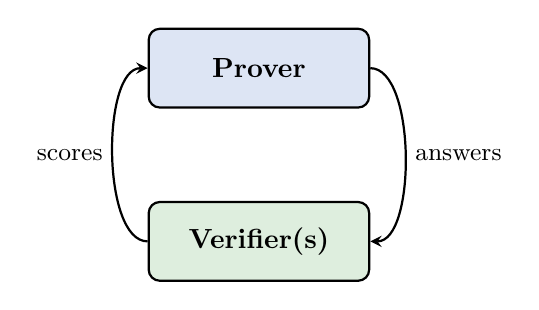
\begin{tikzpicture}[>=stealth, thick]
      \node[draw, rounded corners, fill=midblue!15, minimum width=2.8cm,
            minimum height=1cm] (P) at (0,0) {\textbf{Prover}};
      \node[draw, rounded corners, fill=goodgreen!15, minimum width=2.8cm,
            minimum height=1cm] (V) at (0,-2.2) {\textbf{Verifier(s)}};
      \draw[->] (P.east) .. controls (2,0) and (2,-2.2) .. (V.east)
            node[midway, right] {\small answers};
      \draw[->] (V.west) .. controls (-2,-2.2) and (-2,0) .. (P.west)
            node[midway, left] {\small scores};
    \end{tikzpicture}
  \end{columns}

\end{frame}

% ─── Our Method ───────────────────────────────────────────────────────────────
\begin{frame}{Our Method: A Panel of Small Verifiers + PE-Min}

  \begin{block}{Baseline (Kirchner et al.\ 2024)}
    One large verifier (7B parameters) judges each answer.
    If the prover learns its blind spots, it can reliably fool it.
  \end{block}

  \vspace{0.4em}
  \begin{exampleblock}{Our approach: Multi-Verifier with PE-Min oversight}
    \begin{itemize}
      \item \textbf{3 smaller verifiers} (3B each), each specialised on a different
            aspect: \emph{logical structure}, \emph{computational accuracy},
            \emph{problem alignment}.
      \item The \textbf{PE-Min} rule: the oversight score is learned to approximate
            the \textbf{minimum} across all three verifiers --- the answer must
            convince \emph{every} judge.
      \item Training follows \textbf{Algorithm 1 (Kirchner)}: each round, first
            reset and retrain the aggregator on frozen verifier scores
            (Phase~1a), then train the verifiers via Bradley-Terry pairwise loss
            through the frozen aggregator (Phase~1b).
    \end{itemize}
  \end{exampleblock}

  \vspace{0.3em}
  \textbf{Intuition:} Exploiting one judge's blind spot doesn't help if
  the other two catch you.

\end{frame}

% ─── What we measure ──────────────────────────────────────────────────────────
\begin{frame}{How We Measure Success}

  \begin{columns}
    \column{0.5\textwidth}
    \textbf{Key metrics:}
    \begin{itemize}
      \item \textbf{AUROC} --- How well does the verifier rank correct answers
            above incorrect ones? (1.0 = perfect, 0.5 = random)
      \item \textbf{Separation} --- Average score gap between correct and incorrect
            answers. Bigger = more calibrated.
      \item \textbf{Binary accuracy} --- What fraction of answers does the verifier
            classify correctly?
      \item \textbf{Kirchner attack} --- We fine-tune a fresh prover specifically
            to fool the trained verifier. What fraction of wrong answers does it
            get accepted? Lower = more robust.
    \end{itemize}

    \column{0.46\textwidth}
    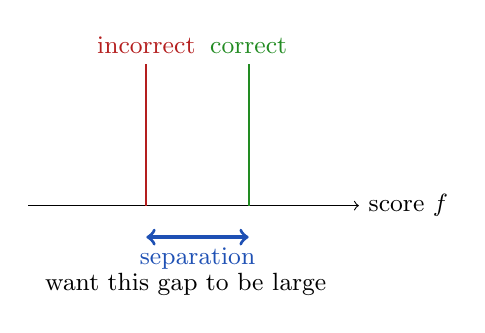
\begin{tikzpicture}
      \draw[->] (0,0) -- (4.2,0) node[right] {\small score $f$};
      \draw[thick, goodgreen] (2.8,0) -- (2.8,1.8)
            node[above] {\small \textcolor{goodgreen}{correct}};
      \draw[thick, badred]   (1.5,0) -- (1.5,1.8)
            node[above] {\small \textcolor{badred}{incorrect}};
      \draw[<->, midblue, very thick] (1.5,-0.4) -- (2.8,-0.4)
            node[midway, below] {\small separation};
      \node at (2.0, -1.0) {\small want this gap to be large};
    \end{tikzpicture}
  \end{columns}

\end{frame}

% ─── Results ──────────────────────────────────────────────────────────────────
\begin{frame}{Results: Supervised Multi-Verifier vs.\ Single-Verifier Baseline}

  \renewcommand{\arraystretch}{1.35}
  \begin{table}
    \centering
    \begin{tabular}{lcc}
      \toprule
      \textbf{Metric} & \textbf{Multi-3B (ours)} & \textbf{Single-7B (baseline)} \\
      \midrule
      AUROC                              & \textcolor{goodgreen}{\textbf{0.827}} & 0.779 \\
      Score separation                   & 0.176 & \textcolor{goodgreen}{\textbf{0.312}} \\
      Binary accuracy                    & \textcolor{goodgreen}{\textbf{73.8\%}} & 72.5\% \\
      Helpful correctness                & \textcolor{goodgreen}{\textbf{42.5\%}} & 40.0\% \\
      \midrule
      CGC attack --- \% wrong accepted   & \textcolor{goodgreen}{\textbf{81.7\%}} & \textcolor{badred}{90.0\%} \\
      SRC attack --- \% wrong accepted   & \textcolor{goodgreen}{\textbf{63.3\%}} & 68.3\% \\
      \bottomrule
    \end{tabular}
    \caption{Lower attack acceptance = harder to fool = better. Both runs use supervised aggregation.}
  \end{table}

  \vspace{0.3em}
  \small
  \textbf{Take-away:} Multi-verifier wins on detection quality (AUROC) and
  is harder to fool under adversarial attack, at the cost of less-calibrated
  absolute scores.

\end{frame}

% ─── PE-Min training dynamics ─────────────────────────────────────────────────
\begin{frame}{PE-Min Training: Early Dynamics (5-Round Run)}

  \begin{columns}
    \column{0.55\textwidth}
    \renewcommand{\arraystretch}{1.25}
    \begin{tabular}{lccc}
      \toprule
      \textbf{Round} & \textbf{BT pairs} & \textbf{Agg loss} & \textbf{Fool rate} \\
      \midrule
      1 & 1   & 0.693 & 0\%  \\
      2 & 62  & 0.690 & 90\% \\
      3 & 149 & 0.269 & ---  \\
      \bottomrule
    \end{tabular}

    \vspace{0.6em}
    \small
    \textit{Agg loss} = Phase~1a H\textsubscript{PE-min} after 3 epochs.\\
    \textit{Fool rate} = fraction of wrong sneaky answers the verifier accepts.\\
    Round~3 collection not yet completed.

    \column{0.42\textwidth}
    \textbf{Observations:}
    \begin{itemize}
      \item Round~1 has almost no same-problem pairs (bootstrap lacks paired
            data) --- verifier signal is near zero.
      \item By Round~3, the replay buffer has 527 records and 149 pairs;
            the aggregator loss drops from 0.61 to 0.27 within 3 epochs.
      \item The two-phase Algorithm~1 is working as intended: verifiers
            receive meaningful gradient signal through the frozen aggregator.
    \end{itemize}
  \end{columns}

\end{frame}

\end{document}
